% intrinsic size and convergence correlations in weak lensing
% Basundhara Ghosh, Ruth Durrer, Bjoern Malte Schaefer

\documentclass[a4paper,fleqn,usenatbib]{mnras}
\usepackage[T1]{fontenc}
\usepackage{ae,aecompl}
\usepackage{graphicx}
\usepackage{amsmath}
\usepackage{amssymb}
\usepackage{txfonts}

\usepackage{float}
\usepackage{adjustbox}

\graphicspath{ {images/} }

\def\spirou#1{{\bf #1}}
\def\foca#1{{\bf #1}}
\def\basundhara#1{{\bf #1}}
\def\ruth#1{{\bf #1}}


% --- macros --- %
\newcommand{\icm}{intra-cluster medium}
\newcommand{\cmb}{cosmic microwave background}


% --- spirou's commands --- %
\newcommand{\ltsima}{$\; \buildrel < \over \sim \;$}
\newcommand{\lsim}{\lower.5ex\hbox{\ltsima}}
\newcommand{\gtsima}{$\; \buildrel > \over \sim \;$}
\newcommand{\gsim}{\lower.5ex\hbox{\gtsima}}
\newcommand{\bra}{\langle}
\newcommand{\ket}{\rangle}
\newcommand{\dang}{d_\mathrm{A}}
\newcommand{\dd}{\mathrm{d}}
\newcommand{\e}{\mathrm{e}}
\newcommand{\p}{\mathrm{p}}

\newcommand{\ci}{\mathrm{i}}
\newcommand{\vecx}{\bmath{x}}
\newcommand{\geo}{\vecx(\btheta,\chip)}
\newcommand{\vecl}{\bmath{\ell}}
\newcommand{\veclp}{\bmath{\ell}^\prime}
\newcommand{\trace}{\mathrm{tr}}
\newcommand{\dlp}{(\ell-\lprime)}

\newcommand{\chip}{{\chi^\prime}}
\newcommand{\chipp}{{\chi^{\prime\prime}}}
\newcommand{\lprime}{\ell^\prime}
\newcommand{\dirac}{\delta_D}
\newcommand{\likeli}{\mathcal{L}}
\newcommand\BG[1]{\textcolor{red}{#1}}

\onecolumn



% --- title --- %
\title[Intrinsic sizes and shapes of galaxies]
{Intrinsic and extrinsic correlations of galaxy shapes and sizes in weak lensing data}
\author[B. Ghosh, R. Durrer, B.M. Sch{\"a}fer]
{Basundhara Ghosh$^1$, Ruth Durrer$^1$, Bj{\"o}rn Malte Sch{\"a}fer$^2$\thanks{e-mail: bjoern.malte.schaefer@uni-heidelberg.de}\\
$^1$D{\'e}partment de la Physique Th{\'e}orique, Universit{\'e} de Gen{\`e}ve, 24 quai Ernest Ansermet, 1211 Gen{\`e}ve, Switzerland\\
$^2$Zentrum f{\"u}r Astronomie der Universit{\"a}t Heidelberg, Astronomisches Rechen-Institut, Philosophenweg 12, 69120 Heidelberg, Germany
}


% --- document --- %
\begin{document}
\pagerange{\pageref{firstpage}--\pageref{lastpage}}
\pubyear{2020}
\maketitle
\label{firstpage}


% --- abstract --- %
\begin{abstract}
The subject of this paper are shape and size correlations of galaxies due to weak gravitational lensing and due to direct tidal interaction of elliptical galaxies with gravitational fields sourced by the cosmic large-scale structure. Setting up a linear intrinsic alignment model that is able to predict intrinsic shape and size correlations in a consistent way we compute the spectra of the intrinsic correlations as well as of the cross-correlations between intrinsic shapes and sizes with weak gravitational shear and convergence, juxtaposing both types of spectra with extrinsic shapes and sizes correlations caused by lensing. We quantify the observability of the intrinsic shape and size correlations and estimate with the Fisher-formalism how well the alignment parameter can be determined from the Euclid weak lensing survey. Specifically, we find a contamination of the weak lensing convergence spectra with an intrinsic size correlation amounting to \spirou{add number}\% over a wide multipole range $\ell=30\ldots300$, with a corresponding cross-correlation exhibiting a sign change, similar to the cross-correlation between weak lensing shear and intrinsic shapes. Quantifying the information content of size correlations in addition to shape correlations shows that bounds can be improved by \spirou{add number}\% for a $w$CDM-cosmology, and that intrinsic correlations decrease the sensitivity of weak lensing due to the negative sign of the cross-correlations by \spirou{add number}. A determination of the alignment parameter yields an precision of $\sigma_D=$\spirou{add number} forecasted for Euclid.
\end{abstract}


% --- keywords --- %
\begin{keywords}
gravitational lensing: weak -- dark energy -- large-scale structure of Universe.
\end{keywords}


lensing 1: \citep{ayaita_investigating_2012,bartelmann_gravitational_2010,bartelmann_weak_2001,bate_when_2019,bernardeau_full-sky_2010,bernstein_comprehensive_2009,bernstein_dark_2004,bernstein_shapes_2002,blazek_beyond_2017,blazek_separating_2012,brainerd_weak_1996,capranico_intrinsic_2013,casarini_non-linear_2011,casarini_tomographic_2012,catelan_intrinsic_2001,chang_dark_2017,cooray_power_2001,cooray_weak_2001,cooray_weak_2002,crittenden_spin-induced_2001,de_jong_kilo-degree_2013,dodelson_weak_2005,dossett_figures_2011,douspis_tension_2019,grandis_information_2016,grassi_detecting_2014,heavens_3d_2003,heavens_combining_2013,heavens_intrinsic_2000,heavens_measuring_2006,heymans_cfhtlens_2013,heymans_weak_2003,hilbert_cosmic_2011,hirata_cross-correlation_2004,hollenstein_constraints_2009,hu_dark_2001,hu_dark_2002,hu_power_1999,hu_power_2001,hu_weak_1999,huff_magnificent_2011}

% --- section:  --- %
\section{introduction}\label{sect_intro}
Weak lensing has emerged as a powerful probe for investigating the cosmic large-scale structure \citep{amara_optimal_2007}, for testing gravitational theories and for constraining cosmological parameters. As gravitational lensing probes fluctuations in the gravitational potential directly, it depends on minimal assumptions and is fixed for a given gravitational theory. Correlations in the shapes of galaxies induced by weak lensing have been detected almost two decades ago, and by now lensing is recognised as a tool for investigating cosmological theories alongside the cosmic microwave background and galaxy clustering. The last generation of surveys, most notably KiDS and DES \citep{Abbott:2017wau} have provided independent confirmation for the $\Lambda$CDM-model and support parameter determinations from the CMB, even though tensions between the two probes, most notably in the matter density $\Omega_m$ and $\sigma_8$ remain. The next generation of surveys, in particular Euclid \citep{Amendola:2016saw} and LSST will probe cosmological models to almost fundamental limits of cosmic variance, but with decreasing statistical errors the control of systematical errors will become one of the central questions for data analysis, along with higher-order effects in the lensing signal related to evaluating the tidal shear fields along a geodesic \citep{Ghosh:2018nsm}, as well as non-Gaussian statistics of the lensing signal due to nonlinear structure formation and non-Gaussian contributions to the covariance.

Among astrophysical contaminants of the weak lensing signal, intrinsic alignments \citep{altay_influence_2006} are perhaps the most dramatic, leading to significant biases in the estimation of cosmological parameters. There are two primary models for the two dominant galaxy types for linking the apparent shapes to tidal gravitational fields in the large-scale structure, which acts, due to long-ranged correlations, as the medium to reduce randomness and to correlate the measured ellipticities. The shapes of spiral galaxies are thought to be determined by the orientation of the angular momentum of the stellar disc \citep{bailin_internal_2005}, and ultimately of the dark matter halo harbouring the stellar component. With this idea in mind, shape correlations are traced back to angular momentum correlations, which in turn would depend through tidal torquing as the angular momentum generated mechanism on the tidal shear fields. Tidal torquing models commonly predict ellipticity correlations on small scales at a level of at most 10\% of the weak lensing signal on multipoles above $\ell\simeq300$ for a survey like Euclid, many physical assumptions have been challenged, most notably the orientation of the disc relative to the host halo angular momentum, as well as an over-prediction of the correlation inherent to the torquing mechanism.

Elliptical galaxies, on the other hand, are thought to acquire shape correlations through direct interaction with the tidal shear field \citep{blazek_beyond_2017, bate_when_2019}: Second derivatives of the gravitational potential would give rise to an anisotropic deformation of the galaxy, in the principal directions of the tidal shear tensor. Interestingly, the reaction of a galaxy to the tidal shear field is determined by the inverse velocity dispersion $1/\sigma^2$ similar to lensing, where the relevant quantity is the gravitational potential in units of $c^2$. Tidal alignments of elliptical galaxies are thought to be present at intermediate angular scales of a few hundred in multipole $\ell$ for a survey like Euclid, with amplitudes being typically an order of magnitude smaller than that of the weak lensing effect. In parallel, alignment models using ideas from effective field theories provide parameterised relationships between tensors constructed from the cosmic density and velocity fields and can capture a wider range of alignment mechanisms and track them into the nonlinear regime, but perhaps with a less clear physical picture. 

While intrinsic alignments refer to a physical change of the appearance of the galaxies, there is an analogous deformation effect on the shape of the light bundle emanating from a galaxy by gravitational lensing. To lowest order, both effects depend on tidal gravitational field which suggests that the effects must be correlated. In fact, cross-correlations between the physical change in shape and the apparent change in shape are predicted to be nonzero for elliptical galaxies, and to be more exact, should in fact be negative as galaxies align themselves radially with a large structure while lensing generates a tangential alignment. As a result, ellipticity correlations of galaxies is a sum of the conventional weak lensing (often referred to as $GG$), the intrinsic alignment (or $II$) and the cross-correlation between the two (called $GI$).

There should be analogous effects of the size of an elliptical galaxy due to tidal gravitational fields: In gravitational lensing the light bundle can be isotropically enlarged, i.e. changed in size while the shape is conserved: This nonzero convergence is caused by the trace of the tidal shear field. Similarly, the size of an elliptical galaxy would physically change for a fixed velocity dispersion if the trace of the tidal shear field is nonzero, or equivalently, if it resides in an overdense or underdense region. An underdense region with density contrast $\delta < 0$ would source a gravitational potential $\Phi$ through the Poisson-equation $\Delta\Phi/c^2 = 3\Omega_m/(2\chi_H^2)\delta$, with the Hubble-distance $\chi_H = c/H_0$, such that the eigenvalues of $\partial_i\partial_j\Phi$ would be negative, stretching the galaxy to a physically larger size. Alternatively, one can argue that the change of volume (or area) is given by the Jacobian of the differential acceleration, i.e. of the tidal shear field, such that $V/V_0 = \mathrm{det}(\delta_{ab} + \partial_a\partial_b\Phi)$, implying that $\ln V-\ln V_0 = \ln\det(\delta_{ab} + \partial_a\partial_b\Phi) = \mathrm{tr}\ln(\delta_{ab} + \partial_a\partial_b\Phi) \simeq \mathrm{tr}(\partial_a\partial_b\Phi) = \Delta\Phi$ and consequently $V/V_0 = \exp(\Delta\Phi)$ and $(V-V_0)/V \simeq\Delta\Phi$.

The motivation of our paper are exactly these correlations between the sizes of elliptical galaxies as they would be predicted by a linear alignment model as a consequence of the trace $\Delta\Phi$ of the tidal shear tensor $\partial_a\partial_b\Phi$ being nonzero. These intrinsic size correlations would be generated in complete analogy to intrinsic shape correlations caused by the traceless part of the tidal shear, and would contaminate measurements of weak lensing convergence correlations \citep{alsing_weak_2014} in the same way as intrinsic shape correlations are a nuisance to the weak lensing shear. After introducing tidal interactions of elliptical galaxies with their surrounding large-scale structure in Sect.~\ref{sect_tidal}, we compute shape correlations from direct tidal interaction and through gravitational lensing in Sect.~\ref{sect_spectra}. We quantify the information content of each of the correlations and the amount of covariance in Sect.~\ref{sect_fisher}, before discussing our results in Sect.~\ref{sect_summary}. In general we work in the context of a $w$CDM-cosmology with a constant equation of state value of $w$ close to $-1$, and standard values for the cosmological parameters, i.e. $\Omega_m = 0.3$, $\sigma_8 =  0.8$, $h = 0.7$ and $n_s = 0.96$, and a parameterised spectrum for nonlinearly evolving scales. We compute numerical results on the information content of size-correlations for the case of a tomographic weak lensing survey like Euclid's \citep{Amendola:2016saw}.


% --- section:  --- %
\section{tidal interactions of galaxies and gravitational lensing}\label{sect_tidal}
In a simplified way one can imagine elliptical galaxies as a stellar component in virial equilibrium with a velocity dispersion $\sigma^2$, filling the gravitational potential. \citet{piras_mass_2018} then argue that if the velocity dispersion is isotropic, one can invoke the Jeans-equation for stationary and static systems in order to relate density $\rho(r)$ and potential $\Phi(r)$,
\begin{equation}
\sigma^2\partial_r\ln\rho(r) = -\partial_r\Phi
\quad\rightarrow\quad
\rho(r) \propto \exp\left(-\frac{\Phi(r)}{\sigma^2}\right),
\end{equation}
reminiscent of the barometric formula. If the gravitational potential is distorted by external fields as the galaxy is not an isolated object, the equipotential contours get distorted correspondingly and the stellar component reacts and galaxy assumes a different shape. To lowest order, the change in shape takes place along the principal axes of the tidal shear tensor $\partial_a\partial_b\Phi$, which is defined as the second derivatives of the gravitational potential $\Phi$,
\begin{equation}
\Phi(r) \rightarrow \Phi(r) + \frac{1}{2}\partial_a\partial_b\Phi\:r_a r_b,
\end{equation}
leading to a distortion of the density of the stellar component. For weak tidal fields, the exponential can be Taylor-expanded to yield
\begin{equation}
\rho \propto 
\exp\left(-\frac{\Phi(r)}{\sigma^2}\right)\left[1-\frac{\partial_a\partial_b\Phi}{2\sigma^2}r_a r_b\right]
\end{equation}
For this perturbed stellar component one can compute the change of the second moments of the brightness distribution, where we ignore projection effects for a moment and use $\rho(r)$ for projected quantities,
\begin{equation}
\Delta q_{cd} = 
\int\dd^2r\:\rho(r)\: r_c r_d\: r_a r_b\times\frac{\partial_a\partial_b\Phi}{2\sigma^2} = S_{abcd}\Phi_{ab},
\end{equation}
which bears a resemblance to the generalised Hooke-law $\Delta q_{cd} = S_{abcd}\Phi_{ab}$, relating the stresses $\Phi_{ab}$ to the observable strains $\Delta q_{cd}$, which suggests to think of $S_{abcd}$ as the susceptibility of a galaxy to change its shape or size under the influence of tidal gravitational fields. In the theory of elastic media one would then in fact use index symmetries to derive that there must be two material constants, similarly, in the theory of viscous fluids one defines two Lam{\'e}-viscosity coefficients (bulk and shear viscosity), so naturally the question arises whether the same constant of proportionality determines the size and the shape deformation as in the case of lensing.

After introducing polar coordinates, assuming spherical symmetry for the unperturbed galaxy and writing $r_0=r\cos\phi$ and $r_1=r\sin\phi$ for the vector components, the elasticity tensor is in our case given by
\begin{equation}
S_{abcd} = 
\frac{1}{2\sigma^2}\int\dd r\:r^5\rho(r)\int\dd\phi\:\cos^{4-(a+b+c+d}\phi\sin^{a+b+c+d}\phi,
\end{equation}
has 16 entries and is fully symmetric under index exchange. Absorbing the prefactor $\int\dd r\:r^5\rho(r)/(2\sigma^2)$ into an alignment parameter $D$, $S_{abcd}$ can only assume three different values, namely $S_{0000} = \int\dd\phi\:\cos^4\phi = S_{1111} = \int\dd\phi\:\sin^4\phi = 3\pi/4$, $S_{0001} = \int\dd\phi\:\cos^3\phi\sin\phi = S_{1110} = \int\dd\phi\:\cos\phi\sin^3\phi = 0$ and $S_{0011} = \int\dd\phi\:\cos^2\phi\sin^2\phi = \pi/4$. 

Introducing the four Pauli-matrices $\sigma^{(n)}_{ab}$ as the basis for the tidal shear $\partial_a\partial_b\Phi$,
\begin{equation}
\sigma^{(0)} = \left(
\begin{array}{cc}
+1 & 0 \\ 0 & +1
\end{array}
\right),~
\sigma^{(1)} = \left(
\begin{array}{cc}
+1 & 0 \\ 0 & -1
\end{array}
\right),~
\sigma^{(2)} = \left(
\begin{array}{cc}
0 & +1 \\ -1 & 0
\end{array}
\right),
\mathrm{~and~}
\sigma^{(3)} = \left(
\begin{array}{cc}
0 & +1 \\ +1 & 0
\end{array}
\right),
\end{equation}
one can determine the change in size $s$ that is introduced by a tidal field $\propto\sigma_{ab}^{(0)}$,
\begin{equation}
s = 
\frac{1}{2}\Delta q_{cd}\sigma^{(0)}_{cd} = 
\frac{1}{2}S_{abij}\sigma^{(0)}_{cd}\sigma^{(0)}_{ab} = 
\frac{1}{2}\left(S_{0000} + S_{0011} + S_{1100} + S_{1111}\right) = 
\pi,
\end{equation}
whereas the change in shape $\epsilon_+$ introduced by a tidal field $\Phi_{ab}\propto\sigma^{(1)}_{ab}$ would be
\begin{equation}
\epsilon_+ = 
\frac{1}{2}\Delta q_{cd}\sigma^{(1)}_{cd} = 
\frac{1}{2}S_{abij}\sigma^{(1)}_{cd}\sigma^{(1)}_{ab} = 
\frac{1}{2}\left(S_{0000} - S_{0011} - S_{1100} + S_{1111}\right) =
\frac{\pi}{2},
\end{equation}
or the change in shape $\epsilon_\times$ generated by the tidal field $\Phi_{ab}\propto\sigma^{(3)}_{ab}$,
\begin{equation}
\epsilon_\times = 
\frac{1}{2}\Delta q_{cd}\sigma^{(3)}_{cd} =
\frac{1}{2}S_{abij}\sigma^{(3)}_{cd}\sigma^{(3)}_{ab} = 
\frac{1}{2}\left(S_{0101} + S_{0110} + S_{1001} + S_{1010}\right) = 
\frac{\pi}{2},
\end{equation}
i.e. the changes in shape are only half as large as the change in size, analogously to the weak lensing convergence with $\Delta\psi = 2\kappa$, which implies as well that the same alignment parameter governs the shape and size distortions. With an assumption on the shape of the projected stellar density $\rho(r)$, for instance a Sersic-profile,
\begin{equation}
\rho(r) \propto \exp\left(-b(n)\left[\left(\frac{r}{r_0}\right)^{1/n}+1\right]\right),
\label{eqn_sersic}
\end{equation}
it is possible to derive the scaling of ellipticity induced by the action of a tidal gravitational field, dominantly with the size of the galaxy but also on the Sersic-index $n$. In eqn.~(\ref{eqn_sersic}), $r_0$ is the scale radius of the stellar component, and $b(n)\simeq 2n - 1/3$, approximatively. Computing the relevant integral $\int\dd r\:r^5\rho(r)$ for a properly normalised density distribution $\int\dd^2r\:\rho(r) = 2\pi\int\dd r\:r\rho(r) = 1$ and using the definition of ellipticity $\epsilon$ as it would result from the second moments $Q_{ab}$ of the normalised brightness distribution $I(r)$,
\begin{equation}
\epsilon = \frac{Q_{xx}-Q_{yy}}{Q_{xx}+Q_{yy}} + 2\ci\frac{Q_{xy}}{Q_{xx}+Q_{yy}},
\quad\mathrm{with}\quad
Q_{ab} = \int\dd^2 r\:I(r)\:r_a r_b,
\end{equation}
where one recognises the size of the image in the denominator, $Q_{xx}+Q_{yy} = \int\dd^2r\:\rho(r)(x^2+y^2) = 2\pi\int\dd r\:r^3\rho$, it is possible to show the scaling of the ellipticity to be
\begin{equation}
\epsilon \propto \frac{\int\dd r\:r^5\rho(r)}{\int\dd r\:r^3\rho(r)} = r_0^2\frac{\int\dd x\:\left(\frac{x}{b}+1\right)^5\exp(-x)}{\int\dd x\:\left(\frac{x}{b}+1\right)^3\exp(-x)},
\end{equation}
obtained after substitution $x = b\left[(r/r_0)^{1/b}-1\right]$, where the ratio of integrals has in general only a numerical solution and shows the dependence of the susceptibility to shape change due to tidal forces caused by the distribution of the stars inside the galaxy. The dominant scaling of ellipticity with the size $r_0^2$ of the galaxy is dimensionally consistent with the linear tidal shear model $Q_{ab} = S_{abcd}\partial_c\partial_d\Phi$. The results are shown in Fig.~\ref{fig_sersic_scaling}, which indicates a strong scaling of the alignment parameter with increasing Sersic-index $n$, where we should note that we consider the Sersic-profile as a reasonably simple model for the stellar distribution, which is not consistent with a constant velocity dispersion $\sigma^2$, and neither a gravitating self-consistent solution. Rather, it is supposed to illustrate that the internal dynamics of an elliptical galaxy can impact on the magnitude of tidal alignment and that not all elliptical galaxies should have the same alignment parameter if their Sersic-index varies.

\begin{figure}
\centering
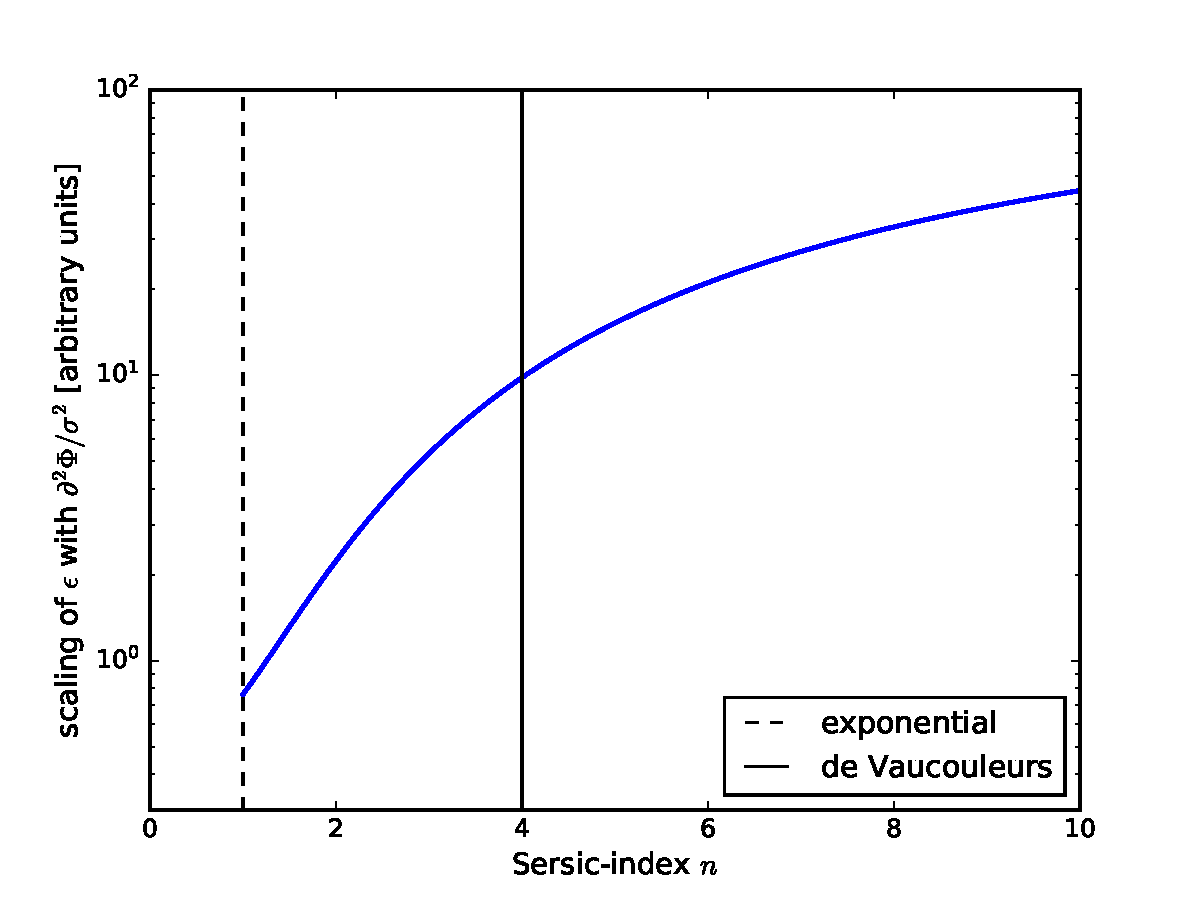
\includegraphics[scale=0.45]{./figures/sersic_scaling.pdf}
\caption{Scaling of the relation between ellipticity $\epsilon$ and Sersic-index $n$, for a given tidal gravitational field and a given velocity dispersion $\sigma^2$. As particular cases, the exponential profile for $n=1$ and the de Vaucouleurs-profile for $n=4$ are indicated by vertical lines.}
\label{fig_sersic_scaling}
\end{figure}

It is straightforward to show that the distortion modes are all independent for the linear model, i.e. tidal fields $\propto\sigma^{(m)}_{ab}$ will never source distortion modes $\propto\sigma^{(n)}_{cd}$ with $m\neq n$. For making the influence of the tidal field on the galaxy size more specific, we compute the change in size $s$ explicitly as the second moment of the brightness distribution for the isotropic case,
\begin{equation}
s = 
\frac{1}{2\sigma^2}\int\dd^2r\:r^2\rho(r)\left[\frac{1}{2}\partial_a\partial_b\Phi\: r_ar_b\right] =
\frac{1}{2\sigma^2}\int\dd^2r\:r^2\rho(r)\left[\frac{1}{4}\Delta\Phi\:r^2\right] = 
\frac{\pi}{\sigma^2}\int r^5\dd r\:\rho(r)\frac{\Delta\Phi}{4} \propto \pi\frac{\Delta\Phi}{2}
\end{equation}
such that the change in size comes out proportional to the trace $\Delta\Phi$ of the tidal field and consistent with the above argumentation with the same definition of the alignment parameter $D$. 

With many galaxies in a tomographic bin $A$ with a suitable, normalised redshift distribution $p_A(z)\dd z$ one can define the line of sight-averaged ellipticity from second angular derivatives of the weighted projection of the potential $\Phi$:
\begin{equation}
\varphi_{A,ab} = \partial_a\partial_b\varphi_A
\quad\mathrm{with}\quad
\varphi_A = D\int\dd\chi\:p_A(z(\chi))\frac{\dd z}{\dd\chi}\frac{D_+}{a}\:\Phi = \int\dd\chi\:W_{\varphi,A}(\chi)\:\Phi,
\label{eqn_ia_los}
\end{equation}
with the Hubble-function $H(\chi)/c = \dd z/\dd\chi$ which originates from the transformation of the redshift distribution, and the growth rate $D_+/a$ of gravitational potentials, and the alignment parameter $D$, which encapsulates the proportionality between tidal shear and physical shape and size change. It would reflect the brightness distribution of a galaxy through its forth moments and scale inversely with the velocity dispersion $\sigma^2$. Because linear intrinsic alignments have the opposite sign compared to gravitational lensing in the same gravitational potential, we choose a negative value for the alignment parameter $D$ in order to not having to carry through minus-signs explicitly. This is due to the fact that an overdense region enlarges the image of a galaxy in lensing but compresses a galaxy physically.

Equation~(\ref{eqn_ia_los}) can be amended to include a bias model, as the galaxy density traces the dark matter density not perfectly. As the intrinsic shape and size-spectra correspond to ellipticity- and diameter-weighted galaxy correlation functions, a biasing model would in fact matter and can change the dependence between the observables and the tidal shear as a function of scale or redshift. For simplicity, we work with a bias of unity without any dependence on mass or redshift, which is reasonable for low-mass galaxies in the relevant redshift range \citep{sheth_large-scale_1999}. Modelling the statistics of the intrinsic alignment effects from a Gaussian random field as we do subsequently ignores that the galaxy shapes and sizes provide a measurement of the tidal field restricted to peak regions of the large-scale structure, which influences the statistics of tidal fields \citep{peacock_statistics_1985, schafer_galactic_2012}.

The angular derivatives $\partial_a$ are related to the spatial derivatives $\partial_x$ through $\partial_a = \chi\partial_x$, with $x=\theta\chi$ in the small-angle approximation. From that, one can recover the ellipticity components $\epsilon_{+,A}$ and $\epsilon_{\times,A}$ as well as the size $s_A$ from a decomposition of the tensor $\varphi_{A,ab}$ with the Pauli-matrices $\sigma_{ab}^{(n)}$,
\begin{equation}
\varphi_{A,ab} = s_A\sigma^{(0)}_{ab} + \epsilon_{+,A}\sigma^{(1)}_{ab} + \epsilon_{\times,A}\sigma^{(3)}_{ab},
\end{equation}
where three components are sufficient because of the symmetry $\varphi_{A,ab} = \varphi_{A,ba}$. Using two properties of the Pauli-matrices $\sigma_{ab}^{(n)}$, namely $\sigma_{ab}^{(l)}\sigma_{bc}^{(m)} = \delta_{lm}\sigma^{(0)}_{ac} + \epsilon_{lmn}\sigma^{(n)}_{ac}$, and their tracelessness $\sigma^{(m)}_{aa} = 0$, it is possible to invert the last relation and to obtain the expansion coefficients,
\begin{equation}
s_A = \frac{1}{2}\varphi_{A,ab}\sigma^{(0)}_{ab},
\quad
\epsilon_{+,A} = \frac{1}{2}\varphi_{A,ab}\sigma^{(1)}_{ab},
\mathrm{~and}\quad
\epsilon_{\times,A} = \frac{1}{2}\varphi_{A,ab}\sigma^{(3)}_{ab}.
\end{equation}

The approach above is motivated by the weak lensing shear $\gamma$, which results from the tensor $\psi_{B,ij}$ containing the second derivatives of the weak lensing potential $\psi_B$,
\begin{equation}
\psi_{B,ij} = \partial_i\partial_j\psi_B
\quad\mathrm{with}\quad
\psi_B = 2\int\dd\chi\:\frac{G_B(\chi)}{\chi}\frac{D_+}{a}\Phi = \int\dd\chi\:W_{\psi,B}(\chi)\Phi,
\end{equation}
with the lensing efficiency
\begin{equation}
G_B(\chi) = \int_{\mathrm{max}(\chi,\chi_B)}^{\chi_{B+1}}\dd\chi^\prime\:p(\chi^\prime)\frac{\dd z}{\dd\chi^\prime}\left(1-\frac{\chi^\prime}{\chi}\right).
\end{equation}
It is interesting to note that the effect of convergence and shear are fully analogous to the changes in size and shape due to direct tidal interaction, up to two details: A light bundle, consisting of photons as relativistic test particles for the gravitational potential, is deflected twice as strongly compared to nonrelativistic test particles such as the stars inside an elliptical galaxies, and the constant of proportionality that makes the gravitational potential dimensionless is $c^2$ in lensing instead of $\sigma^2$ for the intrinsic alignments. We will compute both lensing and intrinsic alignments from the dimensionless potential $\Phi$ give in units of $c^2$ and use a numerical value for the alignment parameter scaled by $c^2/\sigma^2$. Again, there is an analogous decomposition
\begin{equation}
\psi_{B,ij} = \kappa_B\sigma^{(0)}_{ij} + \gamma_{+,B}\sigma^{(1)}_{ij} +\gamma_{\times,B}\sigma^{(3)}_{ij}
\end{equation}
with the analogous inversion,
\begin{equation}
\kappa_B = \frac{1}{2}\psi_{B,ij}\sigma^{(0)}_{ij},
\quad
\gamma_{+,B} = \frac{1}{2}\psi_{B,ij}\sigma^{(1)}_{ij},
\mathrm{~and}\quad
\gamma_{\times,B} = \frac{1}{2}\psi_{B,ij}\sigma^{(3)}_{ij}.
\end{equation}
The intrinsic size field provides a measure of the projected density in the same way as the weak lensing convergence $\kappa$, but with a different weighting function:
\begin{equation}
s = 
\frac{1}{2}\varphi_{ab}\sigma^{(0)}_{ab} = 
\frac{D}{2}\sigma^{(0)}_{ab}\partial_a\partial_b\int\dd\chi\: p(\chi)\frac{D_+}{a}\Phi = 
\frac{D}{2}\int\dd\chi\:p(\chi)\frac{D_+}{a}\chi^2\Delta\Phi = 
\frac{3\Omega_m}{4\chi_H^2}D\int\dd\chi\:p(\chi)\chi^2 \frac{D_+}{a}\delta,
\end{equation}
by substituting the Poisson-equation $\Delta\Phi = 3\Omega_m/(2\chi_H^2)\delta$, using $\partial_a = \chi\partial_x$ for the derivatives, and approximating the full Laplacian by the one containing the derivatives perpendicular to the line of sight. Again, one recognises a factor of two between the gravitational acceleration of photons in gravitational lensing and non-relativistic particles as in our case of stars inside an elliptical galaxy.

This implies that the statistics of all modes of the shape and size field can be described by spectra of the source fields, which in turn are given by a Limber-projection. Specifically, the spectrum of $\varphi_{A,ab}$ reads
\begin{equation}
\bra\varphi_{A,ab}(\bmath\ell)\varphi_{B,ij}^*(\bmath\ell^\prime)\ket = 
(2\pi)^2\dirac(\bmath\ell-\bmath\ell^\prime)\:C^{\varphi_A\varphi_B}_{abij}(\ell)
\quad\mathrm{with}\quad
C^{\varphi_A\varphi_B}_{abij}(\ell) = 
\ell_a\ell_b\ell_i\ell_j\:\int\frac{\dd\chi}{\chi^2}\:W_{\varphi,A}(\chi)W_{\varphi,B}(\chi)\:P_{\Phi\Phi}(k = \ell/\chi),
\end{equation}
similarly, one obtains for the the field $\psi_{B,ij}$,
\begin{equation}
\bra\psi_{A,ab}(\bmath\ell)\psi_{B,ij}^*(\bmath\ell\prime)\ket = 
(2\pi)^2\dirac(\bmath\ell-\bmath\ell^\prime)\:C^{\psi_A\psi_B}_{abij}(\ell)
\quad\mathrm{with}\quad
C^{\psi_A\psi_B}_{abij}(\ell) = 
\ell_a\ell_b\ell_i\ell_j\:\int\frac{\dd\chi}{\chi^2}\:W_{\psi,A}(\chi)W_{\psi,B}(\chi)\:P_{\Phi\Phi}(k = \ell/\chi),
\end{equation}
and finally for their cross-correlation,
\begin{equation}
\bra\varphi_{A,ab}(\bmath\ell)\psi_{B,ij}^*(\bmath\ell^\prime)\ket =
(2\pi)^2\dirac(\bmath\ell-\bmath\ell^\prime)\:C^{\varphi_A\psi_B}_{abij}(\ell)
\quad\mathrm{with}\quad
C^{\varphi_A\psi_B}_{abij}(\ell) =
\ell_a\ell_b\ell_i\ell_j\:\int\frac{\dd\chi}{\chi^2}\:W_{\varphi,A}(\chi)W_{\psi,B}(\chi)\:P_{\Phi\Phi}(k = \ell/\chi).
\end{equation}
In general, all lensing effects originating from a tidal gravitational field will have the opposite sign than the intrinsic tidal alignment, which causes the cross-correlation between lensing and intrinsic alignments to have a negative sign. This is taken care of numerically by choosing a negative value for the alignment parameter $D$, which does not affect the auto-correlations: Those are proportional to $D^2$ and therefore positive. In analogy we define the angular spectra $C^{\varphi_A\varphi_B}(\ell)$, $C^{\psi_A\psi_B}(\ell)$ and $C^{\varphi_A\psi_B}(\ell)$ of the potentials $\varphi_A$ and  $\psi_B$.


% --- section:  --- %
\section{Angular spectra of galaxy shapes and sizes}\label{sect_spectra}
The prefactors $\ell_a\ell_b$ appearing in the expressions for the spectra of the projected tidal shears can be compactly written by introducing polar coordinates, $\ell_0 = \ell\cos\phi$ and $\ell_1 = \ell\sin\phi$. Then,
\begin{equation}
\ell_a\ell_b = 
\frac{\ell^2}{2}\left(\sigma^{(0)}_{ab} + (\cos^2\phi-\sin^2\phi)\sigma^{(1)}_{ab} + 2\sin\phi\cos\phi\sigma^{(3)}_{ab}\right) = 
\frac{\ell^2}{2}\left(\sigma^{(0)}_{ab} + \cos(2\phi)\sigma^{(1)}_{ab} + \sin(2\phi)\sigma^{(3)}_{ab}\right),
\end{equation}
recovering the fact that the phase angle rotates twice as fast as the coordinate system. We are going to make the choice $\phi = 0$ by a suitable rotation of the coordinate frame, such that there are no contractions with $\sigma^{(3)}_{ab}$, and correspondingly vanishing $\gamma_\times$ or $\epsilon_\times$. This corresponds effectively to the computation of $E$- and $B$-modes of the shear field and of the ellipticity field, with
\begin{align}
e(\vecl) = &\hphantom{-}\cos(2\phi)\gamma_+(\vecl) + \sin(2\phi)\gamma_\times(\vecl),\\
b(\vecl) = &-\sin(2\phi)\gamma_+(\vecl) + \cos(2\phi)\gamma_\times(\vecl),
\end{align}
where in our model there are no $B$-modes due to the index exchange symmetry. Now, the decomposition with Pauli-matrices makes it possible to write down all ellipticity spectra as contractions of the the possible spectra of the source terms, for lensing,
\begin{equation}
C^{\gamma\gamma}_{AB}(\ell) = \frac{1}{4}\sigma^{(1)}_{ab}\sigma^{(1)}_{ij}C^{\psi_A\psi_B}_{abij}(\ell) = \frac{l^4}{4}C^{\psi_A\psi_B}(\ell),
\end{equation}
for intrinsic alignments,
\begin{equation}
C^{\epsilon\epsilon}_{AB}(\ell) = \frac{1}{4}\sigma^{(1)}_{ab}\sigma^{(1)}_{ij}C^{\varphi_A\varphi_B}_{abij}(\ell) = \frac{l^4}{4}C^{\varphi_A\varphi_B}(\ell),
\end{equation}
and for the cross-correlation between the two,
\begin{equation}
C^{\epsilon\gamma}_{AB}(\ell) = \frac{1}{4}\sigma^{(1)}_{ab}\sigma^{(1)}_{ij}C^{\varphi_A\psi_B}_{abij}(\ell) = \frac{l^4}{4}C^{\varphi_A\psi_B}(\ell).
\end{equation}
A measurement of the shape correlations is limited by a Poissonian shape noise contribution,
\begin{equation}
N_{AB}^\mathrm{shape}(\ell) = \sigma^2_\mathrm{shape}\frac{n_\mathrm{tomo}}{\bar{n}}\delta_{AB}.
\end{equation}

The extrinsic and intrinsic shape spectra are shown for a tomographic survey in Fig.~\ref{fig:shapeshape}.

\spirou{describe shape correlations}


\begin{figure}
\centering
%
\includegraphics[scale=0.1]{wip.jpg}
\caption{Shape-shape correlations as a function of multipole order $\ell$, separated by gravitational lensing $C_{AB}^{\kappa}(\ell)$, intrinsic size correlations $C_{AB}^{ss}(\ell)$ and the cross-correlation $C_{AB}^{s\kappa}(\ell)$, with the Poissonian noise contribution $N_{AB}^\mathrm{size}(\ell)$ in comparison, for Euclid's redshift distribution and tomography with 5 bins.}
\label{fig:shapeshape}
\end{figure}

In a similar manner like in the previous section, one obtains the size spectra from contracting the possible spectra of the source terms, for lensing,
\begin{equation}
C^{\kappa\kappa}_{AB}(\ell) = \frac{1}{4}\sigma^{(0)}_{ab}\sigma^{(0)}_{ij}C^{\psi_A\psi_B}_{abij}(\ell) = \frac{\ell^4}{4}C^{\psi_A\psi_B}(\ell),
\end{equation}
for intrinsic alignments,
\begin{equation}
C^{ss}_{AB}(\ell) = \frac{1}{4}\sigma^{(0)}_{ab}\sigma^{(0)}_{ij}C^{\varphi_A\varphi_B}_{abij}(\ell) = \frac{\ell^4}{4}C^{\varphi_A\varphi_B}(\ell),
\end{equation}
and again, for the cross-correlation between the two,
\begin{equation}
C^{s\kappa}_{AB}(\ell) = \frac{1}{4}\sigma^{(0)}_{ab}\sigma^{(0)}_{ij}C^{\varphi_A\psi_B}_{abij}(\ell) = \frac{\ell^4}{4}C^{\varphi_A\psi_B}(\ell),
\end{equation}
i.e. all size-spectra are equal to their shape-counterparts. In the estimation process, there is a constant, diagonal noise contribution
\begin{equation}
N_{AB}^\mathrm{size}(\ell) = \sigma^2_\mathrm{size} \frac{n_\mathrm{tomo}}{\bar{n}}\delta_{AB}
\end{equation}

It is straightforward to show that of the 20 possible spectra 10 are in fact nonzero, and that certain consistency relations hold, for instance $\bra\kappa\kappa^\prime\ket = \bra\gamma_+\gamma_+^\prime\ket + \bra\gamma_\times\gamma_\times^\prime\ket$ as well as $\bra ss^\prime\ket = \bra\epsilon_+\epsilon_+^\prime\ket + \bra\epsilon_\times\epsilon_\times^\prime\ket$, in any coordinate frame. Fig.~\ref{fig:sizesize} shows the intrinsic and extrinsic size-spectra, as they would result from a tomographic survey.

\spirou{describe size-correlations}


\begin{figure}
\centering
%
\includegraphics[scale=0.1]{wip.jpg}
\caption{Size-size correlations as a function of multipole order $\ell$, i.e. with gravitational lensing $C_{AB}^{\gamma\gamma}(\ell)$, intrinsic shape correlations $C_{AB}^{\epsilon\epsilon}(\ell)$ and the cross correlation $C_{AB}^{\epsilon\gamma}(\ell)$, with the shape noise contribution $N_{AB}^\mathrm{shape}(\ell)$ in comparison, all for 5-bin tomography with the Euclid galaxy sample.}
\label{fig:sizesize}
\end{figure}


Finally, we compute the cross-correlations between galaxy shapes and sizes, for lensing
\begin{equation}
C_{AB}^{\kappa\gamma}(\ell) = \frac{1}{4}\sigma^{(0)}_{ab}\sigma^{(1)}_{ij}C^{\psi_A\psi_B}_{abij}(\ell) = \frac{l^4}{4}C^{\psi_A\psi_B}(\ell)
\end{equation}
for intrinsic alignments,
\begin{equation}
C_{AB}^{s\epsilon}(\ell) = \frac{1}{4}\sigma^{(0)}_{ab}\sigma^{(1)}_{ij}C^{\varphi_A\varphi_B}_{abij}(\ell) = \frac{\ell^4}{4}C^{\varphi_A\varphi_B}(\ell)
\end{equation}
and for the cross-correlation between lensing and alignments,
\begin{align}
C_{AB}^{\kappa\epsilon}(\ell) & = \frac{1}{4}\sigma^{(0)}_{ab}\sigma^{(1)}_{ij}C^{\psi_A\varphi_B}_{abij}(\ell) = \frac{\ell^4}{4}C^{\psi_A\varphi_B}(\ell)\\
C_{AB}^{s\gamma}(\ell) & = \frac{1}{4}\sigma^{(0)}_{ab}\sigma^{(1)}_{ij}C^{\psi_A\varphi_B}_{abij}(\ell) = \frac{\ell^4}{4}C^{\varphi_A\psi_B}(\ell),
\end{align}
where due to the independence of the errors in the shape and size correlations one does not have to deal with a noise contribution when estimating spectra. Effectively, the cross-correlations between shape and size look identical to the autocorrelations, but in their estimation process there is no noise term, if statistical independence of the two measurement processes is given.


% --- section:  --- %
\section{information content of shape and size correlations}\label{sect_fisher}
For quantifying the information content of intrinsic size and shape correlations in comparison to weak lensing convergence and shear we use the Fisher-matrix formalism. Arranging the measurements of galaxy shapes and sizes into a data vector yields the data covariance matrix,
\begin{equation}
C =
\left(
\begin{array}{cc}
C^{\epsilon\epsilon}_{AB}(\ell) + 2C^{\epsilon\gamma}_{AB}(\ell) + C^{\gamma\gamma}_{AB}(\ell) + N^\mathrm{shape}_{AB} & 
C^{s\epsilon}_{AB^\prime}(\ell) + C^{s\gamma}_{AB^\prime}(\ell) + C^{\kappa\epsilon}_{AB^\prime}(\ell) + C^{\kappa\gamma}_{AB^\prime}(\ell) \\
C^{s\epsilon}_{A^\prime B}(\ell) + C^{s\gamma}_{A^\prime B}(\ell) + C^{\kappa\epsilon}_{A^\prime B}(\ell) + C^{\kappa\gamma}_{A^\prime B}(\ell) & 
C^{ss}_{A^\prime B^\prime}(\ell) + 2C^{s\kappa}_{A^\prime B^\prime}(\ell) + C^{\kappa\kappa}_{A^\prime B^\prime}(\ell) + N^\mathrm{size}_{A^\prime B^\prime}
\end{array}
\right)
\end{equation}
Given the similarities between the shape and size correlations allows to rewrite the covariance matrix as
\begin{equation}
C = \left(
\begin{array}{cc}
\frac{\ell^4}{4}\left(C^{\varphi_A\varphi_B}(\ell)+2C^{\varphi_A\psi_B}(\ell)+C^{\psi_A\psi_B}(\ell)\right) + N^\mathrm{shape}_{AB} & 
\frac{\ell^4}{4}\left(C^{\varphi_A\varphi_{B^\prime}}(\ell)+2C^{\varphi_A\psi_{B^\prime}}(\ell)+C^{\psi_A\psi_{B^\prime}}(\ell)\right)\\
\frac{\ell^4}{4}\left(C^{\varphi_{A^\prime}\varphi_B}(\ell)+2C^{\varphi_{A^\prime}\psi_B}(\ell)+C^{\psi_{A^\prime}\psi_B}(\ell)\right) & 
\frac{\ell^4}{4}\left(C^{\varphi_{A^\prime}\varphi_{B^\prime}}(\ell)+2C^{\varphi_{A^\prime}\psi_{B^\prime}}(\ell)+C^{\psi_{A^\prime}\psi_{B^\prime}}(\ell)\right) + N^\mathrm{size}_{A^\prime B^\prime}
\end{array}
\right),
\end{equation}
which is dangerously close to being singular, underlining the degeneracy between the shape- and size measurements. Already at this stage one should expect that a combined measurement of shear and size does not yield strong improvements of the signal to noise-ratio alone, and given the fact that the same potentials are involved with identical physical dependences on cosmology, resulting Fisher-matrices will be very similar.

The Fisher-matrix $F_{\mu\nu}$ for a tomographic survey assumes the generic form
\begin{equation}
F_{\mu\nu} = f_\mathrm{sky}\sum_\ell\frac{2\ell+1}{2}\mathrm{tr}\left(\partial_\mu\ln C\:\partial_\nu\ln C\right)
\end{equation}
where we implicitly assume a full sky coverage by having independent Fourier-modes, but scale down the Fisher-matrix with the fraction $f_\mathrm{sky} = 0.5$ for the Euclid survey. Similarly, we define the signal to noise ratio $\Sigma$,
\begin{equation}
\Sigma^2 = f_\mathrm{sky}\sum_\ell\frac{2\ell+1}{2}\mathrm{tr}\left(C^{-1}SC^{-1}S\right),
\end{equation}
with the noiseless spectrum $S(\ell)$ of which the signal strength is sought. For the case of Euclid, we extend the summation over the multipoles from $\ell=10$ to $\ell=3000$, and we are assuming for simplicity a full-sky coverage with no correlations between different multipoles, but scale down the signal subsequently with a sky coverage of $f_\mathrm{sky}=0.3$ typical for Euclid, which would be justified because most of the signal originates at small angular scales.

Fig.~\ref{fig:fisher} shows constraints on a $w$CDM-cosmology from galaxy shapes and galaxy sizes.

\begin{figure}
\centering
%
\includegraphics[scale=0.1]{wip.jpg}
\caption{Marginalised $1\sigma$-contours from the Fisher-matrix analysis on a standard $\Lambda$CDM-parameter set, separated by shape correlations and size correlations, with a fixed value of the alignment parameter $D$.}
\label{fig:fisher}
\end{figure}

Fig.~\ref{fig:s2n} quantifies the signal to noise-ratio $\Sigma$ for measuring intrinsic shape and intrinsic size correlations: We compute the signal to noise-ratio for a measurement of the $II$ and $GI$-terms 

\begin{figure}
\centering
%
\includegraphics[scale=0.1]{wip.jpg}
\caption{Signal to noise-ratios $\Sigma$ for Euclid 5-bin tomography for measuring intrinsic shape correlations and for intrinsic size correlations in the presence of weak lensing}
\label{fig:s2n}
\end{figure}


% --- section: summary --- %
\section{summary}\label{sect_summary}
The subject of our investigation were extrinsic and intrinsic shape and size correlations of galaxies due to weak gravitational lensing and intrinsic alignments. 
\begin{itemize}
\item{In a linear alignment model, where}
\end{itemize}
We would like to investigate the usability of both types of shape and size spectra for designing specific tests of gravity, for instance for Vaishtein-type screening mechanisms, which would manifest themselves in differences between the intrinsic and extrinsic shape and size spectra. Likewise, there is the question whether measurements of the velocity dispersion could help to disentangle intrinsic size from lensing shear, as the size effect would cause galaxies with the same velocity dispersion to appear systematically larger in underdense regions, and through velocity dispersion a common baseline could be established. In addition, we would like to point out that the susceptibility $\int\dd r\:r^5\rho(r)$ of a stellar system with density $\rho$ could differ for subclasses of elliptical galaxies giving rise to different effective alignment parameters $D$. Lastly, we would like to comment on possible intrinsic-size and shape effects arising at second order: Similar to lens-lens coupling one could expect a $B$-mode generation if lensing shear acts on a correlated intrinsic ellipticity field \citep[similar to][]{cooray_second-order_2002}, and if lensing deflection shifts the galaxies to new positions \citep{giahi_evolution_2013,giahi-saravani_weak_2014}. 


alignments: \citep{brown_measurement_2002,chisari_contamination_2015,chisari_cosmological_2013,chisari_intrinsic_2014,chisari_intrinsic_2015,chisari_redshift_2016,codis_galaxy_2018,codis_intrinsic_2015,codis_spin_2015,crittenden_spin-induced_2001,debattista_internal_2015,fan_intrinsic_2007,fang_fast-pt_2017,forero-romero_cosmic_2014,fuller_alignments_1999,hall_intrinsic_2014,heavens_bayesian_2016,heavens_combining_2013,heymans_cfhtlens_2013,heymans_weak_2003,heymans_weak_2004,hilbert_intrinsic_2016,hilbert_intrinsic_2017,hirata_galaxy-galaxy_2004,hirata_intrinsic_2007,hirata_intrinsic_2010,jee_cosmic_2015,joachimi_controlling_2010,joachimi_galaxy_2015,joachimi_intrinsic_2010,joachimi_intrinsic_2013,joachimi_simultaneous_2010,johnston_kids+gama:_2018,joudaki_cfhtlens_2017,kasun_shapes_2005,kiessling_galaxy_2015,king_separating_2003,king_suppressing_2002,kirk_galaxy_2015,kirk_optimising_2011,kitching_path_2011,krause_tidal_2011,larsen_intrinsic_2016,lee_alignments_2007,lee_detection_2002,lee_intrinsic_2011,lee_nonlinear_2007,mandelbaum_wigglez_2011,merkel_imitating_2017,merkel_intrinsic_2013,merkel_theoretical_2014,pahwa_alignment_2016,pandya_can_2019,paz_angular_2008,reischke_environmental_2018,schaefer_angular_2015,schaefer_review:_2009,schmitz_time_2018,schneider_galaxy_2013,schneider_halo_2010,taruya_improving_2020,tenneti_galaxy_2014,tenneti_intrinsic_2015,tugendhat_angular_2018,vlah_eft_2019,yao_effects_2017,yao_self-calibration_2018,yao_separating_2019,zhang_spin_2015}


lensing 2: \citep{hui_intrinsic/extrinsic_2002,huterer_calibrating_2005,huterer_nulling_2005,huterer_weak_2002,huterer_weak_2010,jain_cosmological_1997,jain_cross-correlation_2003,jain_ray-tracing_2000,jee_cosmic_2013,jing_intrinsic_2002,joachimi_constraints_2011,joachimi_controlling_2010,joachimi_intrinsic_2010,joachimi_intrinsic_2013,joachimi_removal_2009,kaiser_method_1995,kaiser_weak_1992,kaiser_weak_1998,kayo_cosmological_2013,kayo_information_2013,kilbinger_cfhtlens:_2013,kilbinger_cosmology_2015,kilbinger_dark-energy_2009,kirk_cross-correlation_2015,kirk_impact_2010,kitching_limits_2016,koksbang_accurately_2018,krause_weak_2010,maccrann_cosmic_2014,mackey_theoretical_2002,massey_dark_2010,massey_origins_2013,mellier_probing_1999,mortonson_dark_2013,munshi_cosmology_2008,munshi_principal_2006,munshi_tomography_2014,natarajan_angular_2001,pedersen_first_2019,schaefer_review:_2009,schafer_describing_2016,schafer_weak_2012,schmitz_time_2018,schneider_analysis_2002,sellentin_non-gaussian_2015,semboloni_effect_2013,semboloni_quantifying_2011,shi_controlling_2010,simon_covariance_2004,takada_impact_2009,takada_power_2013,takada_tomography_2004,takahashi_probability_2011,tessore_weak_2015,teyssier_full-sky_2009,thomas_relativistic_2014,troxel_intrinsic_2015,troxel_self-calibration_2012,valageas_source-lens_2014,valageas_statistical_1999,van_waerbeke_efficiency_1999,van_waerbeke_weak_2001,vanderveld_neutrino_2013,vanderveld_second-order_2011,vanderveld_testing_2012,white_baryons_2004,yu_fast_2016}


spin:\citep{bailin_internal_2005,dubinski_cosmological_1992,goldberg_spins_1967,pahwa_alignment_2016,paz_angular_2008,peebles_origin_1969,schafer_galactic_2012,white_angular_1984}




% --- section: acknowledgements --- %
\section*{Acknowledgements}
BG thanks...   BMS likes to thank the Universidad del Valle in Cali, Colombia, for their kind hospitality. We thank Jolanta Zjupa for spotting a mistake in an early version of the draft.


% --- bibliography --- %
\bibliographystyle{mnras}
\bibliography{references}


\bsp
\label{lastpage}
\end{document}
